% -*- mode: latex; mode: auto-fill; -*-
\section{Ambient Occlusion}

Ambient Occlusion is a popular technique for approximating soft
shadows in a scene. The technique deals only with the kind of light
that is scattered in all directions (ambient light) and as such no
particular light source is taken into consideration. In other words
ambient occlusion assumes a global illumination of uniform intensity
and is completely independent of light sources.
The intensity of the ambient light on a particular point on a
three-dimensional surface is determined by the overall occlusion due
to geometrical objects in the vicinity of the point. In general the
ambient occlusion of a three-dimensional point $\mathbf{P}$ with
surface normal $\hat{n}$ can be described by the following equation
\citep{shanmugam}:
\begin{equation}
  \label{eq:ao}
  A(\mathbf{P},\hat{n}) = \frac{1}{\pi} \int_\Omega V(\hat{\omega},\mathbf{P})\max(\hat{\omega}\cdot\hat{n},0)\,\mathrm{d}\hat{\omega}
\end{equation}
where we integrate over every direction within a fixed radius
hemisphere $\Omega$ centered in the point $\mathbf{P}$ with the zenith
axis pointing in the direction of the surface normal $\hat{n}$. $V$ is
a function that returns $1$ if any geometrical object is intersected
when tracing from $\mathbf{P}$ in the direction of $\hat{\omega}$ and
$0$ otherwise. The resulting value lies on the interval $[0,1]$ and
represents a weighted average of every direction within the
hemisphere. Each weight is dependent on the angle between the normal
$\hat{n}$ and the direction $\hat{\omega}$ and ensures that object
intersections with large angles contributes with less occlusion than
intersections in a direction which is closer to the direction of the
surface normal.

For better results one can extend equation (\ref{eq:ao}) with an
attenuation function to account for the distance between $\mathbf{P}$
and an the occluding object. This would yield
\begin{equation}
  \label{eq:ao_att}
  A(\mathbf{P},\hat{n}) = \frac{1}{\pi} \int_\Omega
  V(\hat{\omega},\mathbf{P})\max(\hat{\omega}\cdot\hat{n},0)W(R,r) \,\mathrm{d}\hat{\omega}
\end{equation}
where $R$ is the hemisphere radius and $r$ is the distance between
$\mathbf{P}$ and the occluding object. For instance $W$ could be
defined as the quadratic attenuation function scaled by the hemisphere
radius given by
\begin{equation}
  \label{eq:quad_att}
  W(R,r) = 1-\left(\frac{r}{R}\right)^2
\end{equation}

\subsection{Screen Space Ambient Occlusion}
\label{sec:ssao}
Ambient occlusion as described in the above could be done by tracing a
finite number of rays for a discretized set of points on each planar
surface and performing intersection tests with nearby
geometry. Obviously this is a computationally expensive approach which
would not work in real-time rendering. Also it would be wasteful to
perform the calcutions described in (\ref{eq:ao}) and
(\ref{eq:ao_att}) on every planar surface in the scene since only a
very small number surfaces are actually visible in the final image.

Screen space ambient occlusion \citep{ssao} is a fast technique for
approximating ambient occlusion as previously described. The algorithm
is completely independent of scene geometry as it uses the depth
buffer as a rough approximation of the visible geometry. Assuming that
the depth buffer is available together with a buffer containing the
surface normals given in eye-space coordinates of the geometry
behind each fragment, this technique can be viewed as a geometry
independent post-processing effect. As a result the complexity of the
algorithm only depends on the resolution of the screen.

The basic idea behind screen space ambient occlusion is that the depth
buffer can be viewed as a height map depicting the curvature of
all the front-most visible geometry with respect to the eye
position. Each two-dimensional position on the screen surface
can then be translated into a three-dimensional point in screen space by
means of the depth value. A finite number of rays within the hemisphere
in the direction of the surface normal can then be traced using a
technique called ray-marching. Ray-marching traces a ray by stepping
along the direction of the ray. The step size is a fixed predermined
value. Occluders are then detected by testing intersections with the
height map determined by the depth buffer.
\todo{describe unprojection}

\subsection{Horizon-based Ambient Occlusion}
\label{sec:hbao}
A further performance improvement is achieved by realising that
ray-marching in eye-space is unnecessary since our input data is
two-dimensional \citep{hbao}. This is the underlying observation of
the horizon-based ambient occlusion approach, where we trace entirely
in image-space. For each fragment in the image plane we unproject the
corresponding three-dimensional point $\mathbf{P}$ as described in
section \ref{sec:ssao}. We then approximate the hemisphere by
projecting a sphere centered in $\mathbf{P}$ back onto the image
plane. On the resulting two-dimensional circle we randomly pick a
finite number of uniformly distributed two-dimensional directions. In
each of these directions we now determine a horizon line by stepping
in image-space and compare depth values along the way. The horizon
line is then given by the vector going from $\mathbf{P}$ to the
highest point on the height map along the traced line. The point is
obtained by unprojecting the two-dimensional point with the lowest
depth value as was done with the point $\mathbf{P}$. The concept of
the horizon line is illustrated in figure \ref{fig:horizon}.
\begin{figure}[h]
  \centering
  tis
  \caption{Horizon stuff.}
  \label{fig:horizon}
\end{figure}
To obtain an occlusion measure in a given direction we compare the
the horizon with the surface normal $\hat{n}$ in the point
$\mathbf{P}$. This is done in the following way.

\subsection{Applying the Ambient Occlusion Map}

\subsection{Implementation}

We have implemented a variant of the horizon-based ambient occlusion
using a simple gaussian blur kernel for smoothing the ao map.  The
algorithm is divided into a number of stages represented by a specific
shader program for each stage. Some of these stages could be collapsed
into a single shader but we have chosen this strategy in order to
toggle each phase on and off at run-time.

The entire implementation resides in a post-process module wich has
been attached to the OpenEngine renderer. The module will receive an
event whenever the renderer has completed its main rendering phase. It
is then safe to assume, that the back buffer contains the rendered
scene.  The first thing we do is to store this image in a texture for
later use. This is done in the following OpenGL code:
\begin{cppcode}
  glBindTexture(GL_TEXTURE_2D, scene);
  glCopyTexImage2D(GL_TEXTURE_2D, 0, GL_RGB, 0, 0, width, height, 0);
  glBindTexture(GL_TEXTURE_2D, 0);
\end{cppcode}

In the following we list the different stages comprising our ambient
occlusion effect.

\subsubsection*{Initializing the ambient occlusion module}
Our module will also receive an event from the OpenEngine renderer
upon initialization, and at this point it is safe to assume that
an OpenGL context has been initialized. We can then start to
initialize the neccessary OpenGL structures which consists of a
framebuffer to use as a render target for intermediate textures. The
following textures are attached to the frame buffer:
\begin{itemize}
\item A three channel 32 bit floating point texture for storing the
  surface normals;
\item a depth texture for storing the z-values of the rendered scene;
\item a single channel 32 bit floating point texture for storing the
  ambient occlusion map;
  \item and a single channel 32 bit floating point texture for storing the
  result of the gaussian blur kernel.
\end{itemize}
We then load and compile the relevant shaders using OpenEngine's
shader resource manager. We use the following shaders:
\begin{itemize}
\item A normalshader for generating surface normals;
\item the ambient occlusion shader for generating the ambient
  occlusion map;
\item two gaussian blur shaders one for bluring in the x-direction and
  one for the y-direction;
\item and a simple merge shader for combining the ambient occlusion
  map with the pixels from the original scene.
\end{itemize}

\subsubsection*{Collecting normals and depth values}  
Since our only assumption is that the source image lies in the frame
buffer, it is now possible to overlay an arbitrary scene with ambient
occlusion in a post-render phase. This also means that we have to
generate all the surface normals and depth values before we can
produce the ambient occlusion map. We do this by traversing the scene
graph and rendering all scene geometry with our normal shader
applied. The following lines of code initiates the rendering of the normals.
\begin{cppcode}
  // bind normal vector frame buffer texture
  glBindFramebufferEXT(GL_FRAMEBUFFER_EXT, fbo);
  glDrawBuffer(GL_COLOR_ATTACHMENT0_EXT);
  
  glEnable(GL_DEPTH_TEST);
  glDisableClientState(GL_VERTEX_ARRAY);
  glDisableClientState(GL_NORMAL_ARRAY);
  glDisableClientState(GL_COLOR_ARRAY);
  glClearColor(0.0,0.0,0.0,1.0);
  glClear( GL_COLOR_BUFFER_BIT | GL_DEPTH_BUFFER_BIT );
  
  // collect normals 
  normalShader->ApplyShader();
  CHECK_FOR_GL_ERROR();
  arg.canvas.GetScene()->Accept(*this);
  CHECK_FOR_GL_ERROR();
  normalShader->ReleaseShader();
\end{cppcode} 
The body of the vertex shader is given below
\begin{cppcode}
  eyePos = (gl_ModelViewMatrix * gl_Vertex).xyz;
  gl_Position = ftransform();
  normal = normalize(gl_NormalMatrix * gl_Normal);
\end{cppcode}
This is a standard vertex shader transforming the vertex and the
vertex normal into eye space. The interesting part lies in the
fragment shader which is given by the oneliner below
\begin{cppcode}
  gl_FragColor.rgb = normalize(cross(dFdx(eyePos), dFdy(eyePos)));
\end{cppcode}
This is a nice trick for producing the correct surface
normals instead of the interpolated ones. Here we compute the
derivatives of the varying vertex coordinates in eyespace
with respect to x and y, respectively. The cross product between these
vectors is then a new vector perpendicular to the original triangle
given in eye space coordinates, hence a surface normal. Figure
\ref{fig:normals} illustrates the difference between the surface
normals and the interpolated vertex normals.

\begin{figure}[h]
  \centering
  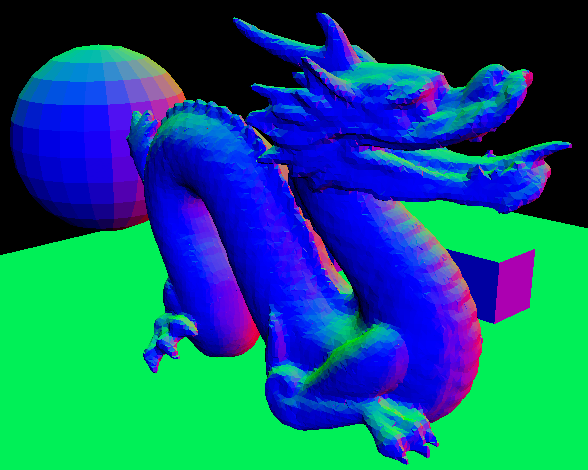
\includegraphics[width=6cm]{hardnormals}
  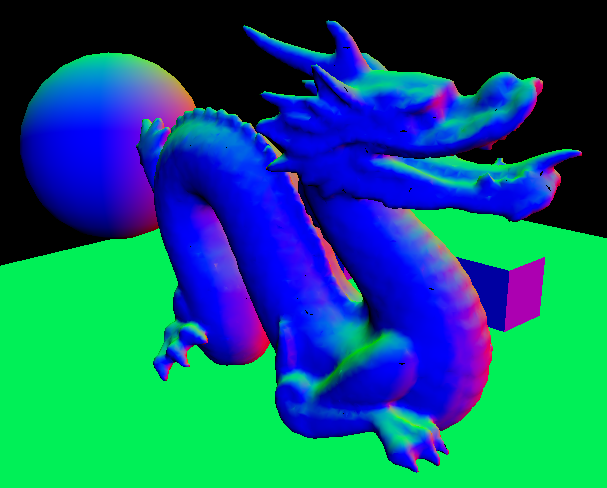
\includegraphics[width=6cm]{softnormals}
  \caption{Rendering of the normal map. To the left: Using hard
    normals. To the right: Using interpolated vertex normals.}
  \label{fig:normals}
\end{figure}
\subsubsection*{Producing the ambient occlusion map}  
When the surface normals and the depth buffer have been obtained in
textures, we can proceed with the actual ambient occlusion
algorithm. The algorithm is written in a single shader and operates on
each pixel of the normal and depth textures. In order to activate the
shader we simply draw a quad where each vertex has uv coordinates
$(0,0), (0,1), (1,1), (1,0)$, respectively. The vertex coordinates are
unimportant since we calculate these from the uv coordinates in the
vertex shader. The body consists of the following two lines
\begin{cppcode}
  uv = gl_MultiTexCoord0.xy;
  gl_Position = vec4((uv * 2.0) - vec2(1.0,1.0), 0.0, 1.0);
\end{cppcode}
which simply transform the uv coordinates lying in $[0,1]$ into window
coordinates lying in $[-1,1]$.

The fragment shader is where all the heavy work is carried out. There
several uniforms which affects the resulting output. First of all the
following uniforms are required
\begin{cppcode}
  uniform sampler2D normals;
  uniform sampler2DShadow d;
  uniform mat4 proj;
  uniform mat4 unproj;
\end{cppcode}
where the first two lines are the surface normal texture and the depth
buffer texture. The third line is the projection matrix used to render
the original scene and the last line is the inverted projection
matrix. These two matrices are used for converting between window
coordinates and eye-space coordinates. This is done in the following
helper functions
\begin{cppcode}
  vec3 unproject(vec2 pos, float depth) {
    vec4 res = unproj * vec4(pos, depth, 1.0);
    return res.xyz / res.w;
  }
  
  vec2 project(vec3 pos) {
    vec4 res = proj * vec4(pos, 1.0);
    return res.xy / res.w;
  }
\end{cppcode}

Next we have the following user definable variables to affect the
behaviour of the algorithm.
\begin{cppcode}
  uniform float sphereRad;
  uniform float contrast;
  uniform float rays;
  uniform float steps;
  uniform float bias;
\end{cppcode}
These variables represent
\begin{itemize}
\item the radius of the sphere in which to search for occluders,
\item the contrast of the shadows,
\item the number of rays to trace in image space,
\item the number of steps to take when sampling in each ray direction,
\item the angle bias, 
\end{itemize}
respectively.

We first project the sphere radius onto the image plane. This is done
by the following line of code
\begin{cppcode}
  float circleRad = length(winPos - project(fragPos + vec3(sphereRad, 0.0, 0.0))); 
\end{cppcode}
where winPos is the window position of the current fragment and
fragPos is the unprojection of winPos.  The main part of the algorithm
consists of an outer for loop iterating over the number of rays. The
angles of the rays are uniformly distributed. An inner loop then
traces each ray by taking a predefined number of steps on the ray and
unproject each two-dimensional position on the way. The inner loop
looks as follows
\begin{cppcode}
  for (float j = 0.0; j < steps; j = j + 1.0) {
    pos += stepRay;
    vec3 new = unproject(pos, shadow2D(d, vec3(win2uv(pos), 0.0)).x);
    if (new.z < horizon.z) {
      horizon = new;
    }
  }
\end{cppcode}
where pos has been initialized to the window position of the current
fragment and stepRay is a two-dimensional vector pointing in the
direction of the current ray and has length corresponding to the
circle radius normalized by the number of steps. When the loop
terminates the horizon vector should contain the eye space position of
the ``highest'' point on the height map defined by the depth
buffer. The actual horizon line can then be computed by
\begin{cppcode}
  horizon = horizon - fragPos;
\end{cppcode}
We now have the information to compute the contribution measure as
described in section \ref{sec:hbao}. This is done in the following lines
\begin{cppcode}
  // calculate tangent to the surface normal
  horizon = normalize(horizon);
  vec3 tan   = vec3(1,0,0);
  vec3 bitan = normalize(cross(normal, tan));
  tan        = normalize(cross(bitan, normal));
  
  // calculate angles in [-PI; PI]
  float hAngle = atan(horizon.z / length(horizon.xy));
  float tAngle = atan(tan.z / length(tan.xy)) + bias;
  
  // final ao contribution of this direction
  ao += (sin(hAngle) - sin(tAngle));
\end{cppcode}
where the upper part calculates the tangent to the surface normal, the
middle part places the angles in the interval $[-\pi,\pi]$, and the
last line accumulates the occlusion measure.

When we are done accumulating the occlusion contributions from each
ray we produce a final output value by averaging over the number of
rays.
\begin{cppcode}
  gl_FragColor = vec4(1.0 - (ao/rays) * contrast);
\end{cppcode}
We now have a value that will shade the corresponding pixel in the
original scene image by multiplying the two values.

\subsubsection*{Applying the ambient occlusion map}
Before applying the ambient occlusion map, we perform a simple gaussian
blur to soften the shadows. This is done in two stages, first a blur
in the x-direction and then a blur in the y-direction. We use the same
technique of drawing a quad as before to activate the shaders. The
shaders themselves are pretty much self-explanatory so it is
unnecessary to cover them in further detail. An important thing to
mention is that the gaussian blur should be replaced with a bilateral
filter, that would account for large differences in depth values to
avoid bleeding across edges. The result of the blur kernel is finally
combined with the original image by multiplication of the pixel value
with the corresponding ambient occlusion value. This is done in a very
simple one-line shader.

\subsection{Results}

The result of our ambient occlusion shader can be seen in figure
\ref{fig:res}. 

\begin{figure}[h]
\label{fig:res}
  \centering
  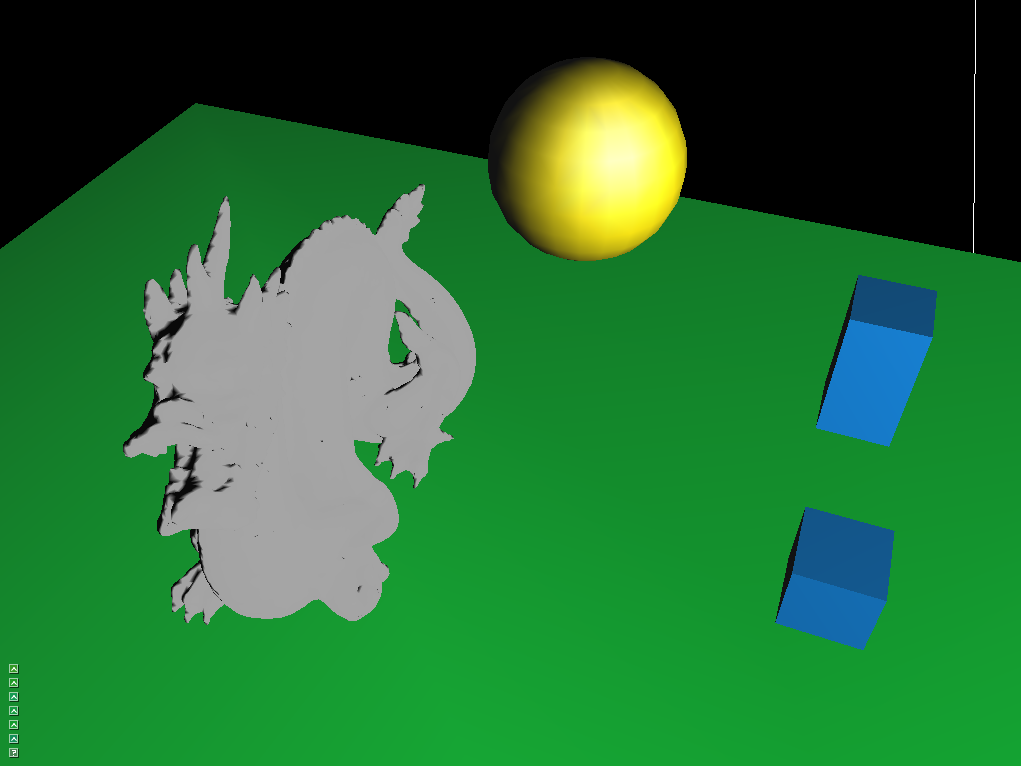
\includegraphics[width=6cm]{noao}
  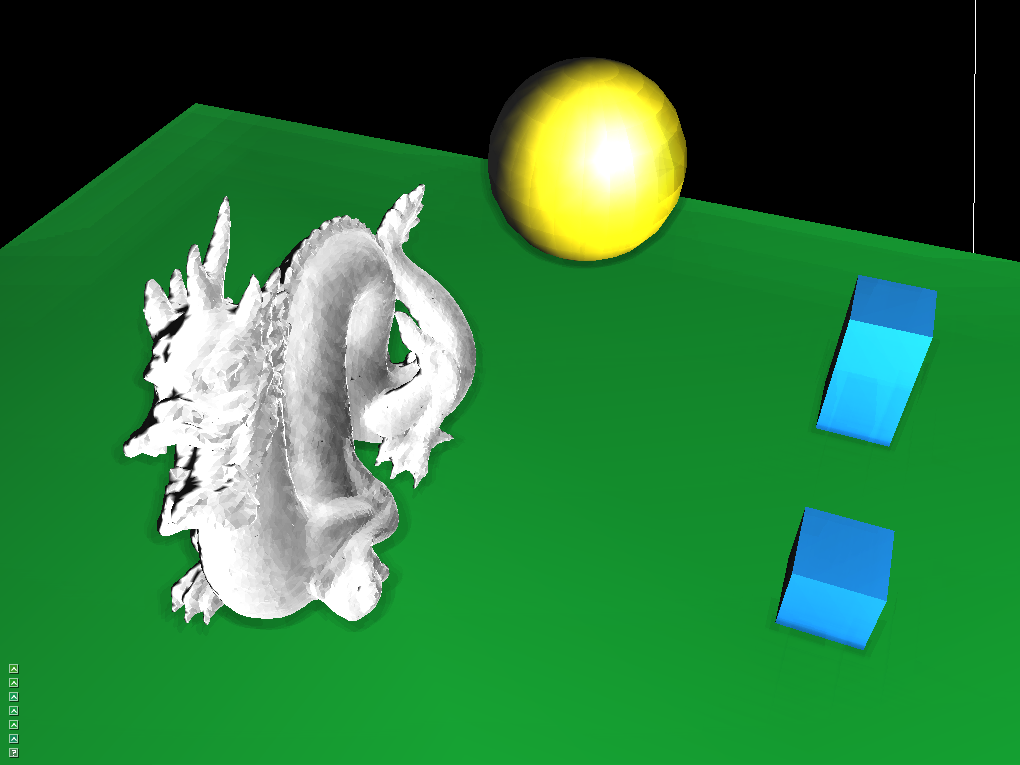
\includegraphics[width=6cm]{aonoblur}
  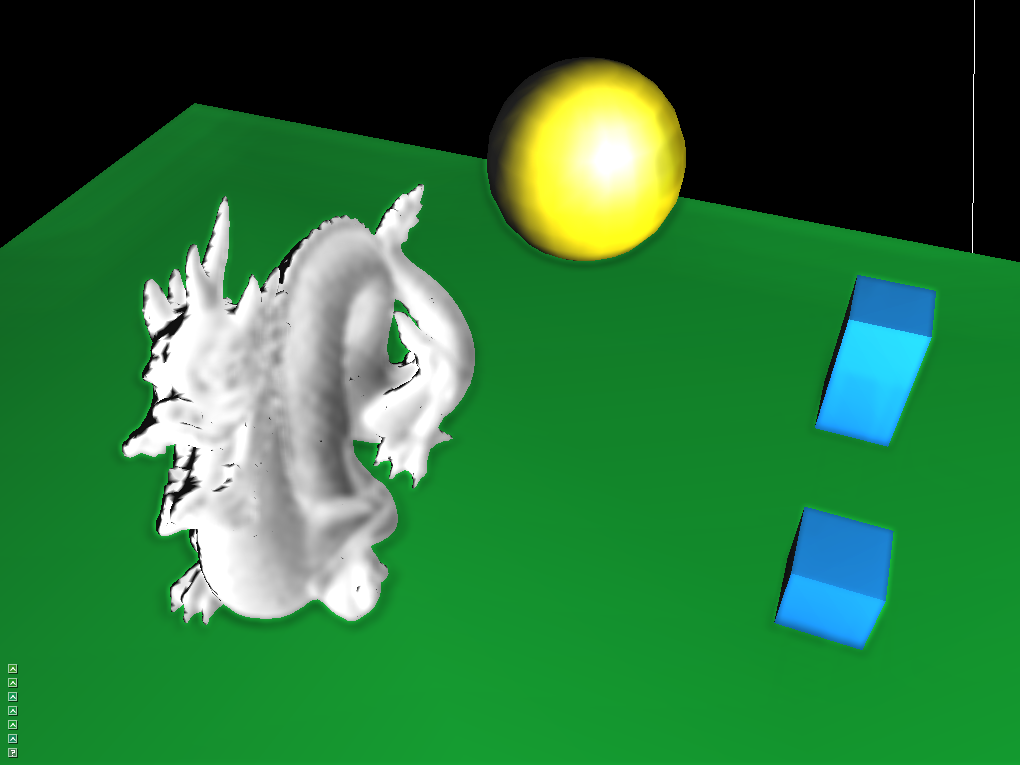
\includegraphics[width=6cm]{aoblur}
  \caption{Our ambient occlusion at work. Upper left: Without ambient
    occlusion. Upper right: With ambient occlusion but no blur
    kernel. Bottom: With both ambient occlusion and gaussian blur kernel.}
\end{figure}

%%% Local Variables: 
%%% mode: latex
%%% TeX-master: "master"
%%% End: 
